% Haar wavelet decomposition diagram showing signal and wavelets at each resolution level
% Arranged in a 2x2 grid to fit in a single column
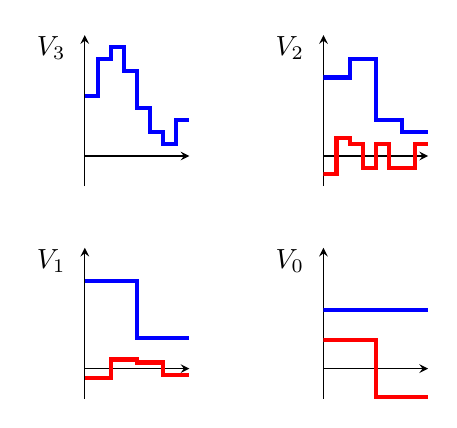
\begin{tikzpicture}
  % Top row: Resolution 8 (V_3) - top left
  \begin{axis}[
    at={(0.13\textwidth,4.5cm)},
    width=0.24\textwidth,
    height=3.5cm,
    xmin=0, xmax=1,
    ymin=-2.5, ymax=10,
    ytick=\empty,
    xtick=\empty,
    axis x line=middle,
    axis y line=center,
  ]
    \addplot[const plot, line width=1.5pt, color=blue] coordinates {
      (0,5) (0.125,5) (0.125,8) (0.25,8) (0.25,9) (0.375,9) (0.375,7) (0.5,7) (0.5,4) (0.625,4) (0.625,2) (0.75,2) (0.75,1) (0.875,1) (0.875,3) (1,3)
    };
  \end{axis}
  \node[anchor=east] at (0.12\textwidth, 6.25cm) {$V_3$};
  
  % Top row: Resolution 4 (V_2) - top right
  \begin{axis}[
    at={(0.38\textwidth,4.5cm)},
    width=0.24\textwidth,
    height=3.5cm,
    xmin=0, xmax=1,
    ymin=-2.5, ymax=10,
    ytick=\empty,
    xtick=\empty,
    axis x line=middle,
    axis y line=center,
  ]
    \addplot[const plot, line width=1.5pt, color=blue] coordinates {
      (0,6.5) (0.25,6.5) (0.25,8) (0.5,8) (0.5,3) (0.75,3) (0.75,2) (1,2)
    };
    \addplot[const plot, line width=1.5pt, color=red] coordinates {
      (0,-1.5) (0.125,-1.5) (0.125,1.5) (0.25,1.5) (0.25,1) (0.375,1) (0.375,-1) (0.5,-1) (0.5,1) (0.625,1) (0.625,-1) (0.75,-1) (0.75,-1) (0.875,-1) (0.875,1) (1,1)
    };
  \end{axis}
  \node[anchor=east] at (0.37\textwidth, 6.25cm) {$V_2$};

  % Bottom row: Resolution 2 (V_1) - bottom left
  \begin{axis}[
    at={(0.13\textwidth,1.8cm)},
    width=0.24\textwidth,
    height=3.5cm,
    xmin=0, xmax=1,
    ymin=-2.5, ymax=10,
    ytick=\empty,
    xtick=\empty,
    axis x line=middle,
    axis y line=center,
  ]
    \addplot[const plot, line width=1.5pt, color=blue] coordinates {
      (0,7.25) (0.5,7.25) (0.5,2.5) (1,2.5)
    };
    \addplot[const plot, line width=1.5pt, color=red] coordinates {
      (0,-0.75) (0.25,-0.75) (0.25,0.75) (0.5,0.75) (0.5,0.5) (0.75,0.5) (0.75,-0.5) (1,-0.5)
    };
  \end{axis}
  \node[anchor=east] at (0.12\textwidth, 3.55cm) {$V_1$};
  
  % Bottom row: Resolution 1 (V_0) - bottom right
  \begin{axis}[
    at={(0.38\textwidth,1.8cm)},
    width=0.24\textwidth,
    height=3.5cm,
    xmin=0, xmax=1,
    ymin=-2.5, ymax=10,
    ytick=\empty,
    xtick=\empty,
    axis x line=middle,
    axis y line=center,
  ]
    \addplot[const plot, line width=1.5pt, color=blue] coordinates {
      (0,4.875) (1,4.875)
    };
    \addplot[const plot, line width=1.5pt, color=red] coordinates {
      (0,2.375) (0.5,2.375) (0.5,-2.375) (1,-2.375)
    };
  \end{axis}
  \node[anchor=east] at (0.37\textwidth, 3.55cm) {$V_0$};

\end{tikzpicture}

